En este laboratorio se introduce al mundo de las nanopartículas con la sintetización de compuestos con plata $AgNPs$ con la intención de evaluar su estabilidad ante diferentes condiciones de pH y concentración de sales, de esta manera completar el estudio de los mismos en el laboratorio.

\textbf{\textcolor{azul50}{Formalismo}}

Las nanotecnologías aprovechan las propiedades excepcionales de partículas que se miden a escalas nanométricas, conocidas comúnmente como nanopartículas.  La nanotecnología se encarga del diseño, producción y empleo de estructuras y objetos a escala nanométrica. Los conocimientos actuales sobre la nanociencia provienen de avances en los campos de la química, física, biología, medicina e ingeniería entre otras. En la ciencia de materiales, las nano partículas permiten la fabricación de productos con propiedades mecánicas nuevas, incluso en termino de superficie de rozamiento, de resistencia al desgaste y de adherencia. En biología y medicina, los nanomateriales se emplean en la mejora del diseño de fármacos y su administración dirigida. En el campo de la electrónica se emplean en el diseño de dispositivos de almacenamiento de datos de menor tamaño, más rápido y con menor consumo de energía. 

A menudo las nanopartículas cuentan con propiedades físicas y químicas muy diferentes a las de los mismos materiales a escala macroscópica. Sus propiedades dependen de su forma y tamaño, características de superficie y estructura interna. La presencia de ciertas sustancias químicas también puede alterar dichas propiedades. Los parámetros principales de las nanopartículas son su forma, el tamaño y la subestructura morfológica de las sustancias. Presentan una suspensión en su mayoría solida en líquidos o una emulsión. En presencia de agentes químicos las propiedades superficiales e interfaciales pueden ser modificadas. Tales agentes pueden estabilizarse contra la coagulación o la agregación conservando la carga de las partículas y modificando su la capa más externa. Dependiendo de la historia de crecimiento y vida útil de una nanopartícula, deben esperarse composiciones muy complejas, en la historia típica de una nanopartícula de combustión, por ejemplo, muchos agentes diferentes son propensos a la condensación de la partícula mientras se enfría y se expone a diferentes ambientes y atmosferas. 

En la nanoescala , las interacciones partícula-partícula están dominadas por fuerzas débiles de Van der Waals, interacciones polares y electrostáticas más fuertes o interacciones covalentes. Dependiendo de la viscosidad y la polarización del fluido, la agregación de partículas está determinada por la interacción entre partículas. Mediante la modificación de la capa superficial, la tendencia de un coloide a coagularse puede aumentar u obstaculizarse. Para las nanopartículas suspendidas en el aire, las cargas pueden acumularse mediante procesos físicos como descarga luminiscente o fotoemisión. En líquidos, carga de partículas. Puede ser estabilizado por procesos electroquímicos en las superficies. Los detalles de las fuerzas de interacción nanopartícula - nanopartícula y las interacciones nanopartícula - fluido son de importancia clave para describir los procesos físicos y químicos, y la evolución temporal de las nanopartículas libres. Siguen siendo difíciles de caracterizar debido a la pequeña cantidad de moléculas. Participa en la capa de superficie activa. Tanto la energía superficial, la carga y la solvatación son parámetros relevantes para considerar. Debido al papel crucial de la interacción nanopartícula - nanopartícula y la interacción nanopartícula - fluido, el término nanopartícula libre puede ser mal interpretado fácilmente. Las fuerzas de interacción ya sean atractivas o repulsivas, determinan crucialmente el destino de las nanopartículas individuales y colectivas. Esta interacción entre nanopartículas que resulta en agregados y / o aglomerados puede influir en su comportamiento. En las suspensiones de gas, la agregación se determina de manera crucial por el tamaño y la difusión, y la coagulación suele ocurrir más rápido que en la fase líquida, ya que el coeficiente de adherencia es más cercano a la unidad que en los líquidos.

Las nanopartículas metálicas han sido de gran interés debido a sus propiedades físicoquímicas, tamaño y comportamiento de los plasmones de superficie, entre las mas usadas encontramos las nanopartículas de plata ($AgNPs$), se han utilizado en diversos ámbitos como la optoelectrónica, biosensores además de otras. Una de las propiedades mas explotada a sido la naturaleza antimicrobiana de la plata. se ha demostrado mediante estudios que la naturaleza microbiana de es dependiente del tamaño y la forma de las nanopartículas, las mas pequeñas tienen una mejor respuesta antimicrobiana. Referente a la forma las nanopartículas con forma esférica se consideran las mas adecuadas para aplicaciones practicas en forma coloidal. 

Con pocas excepciones, la reducción mediada por borohidruro se ha empleado para la síntesis de nanopartículas de plata dispersables. Para nanopartículas de pequeño tamaño, un exceso de agente reductor fuerte, por ejemplo, borohidruro de sodio Se desea (NaBH4), lo que facilita la generación de núcleos instantáneos, lo que resulta en la formación de coloides de plata de tamaño uniforme y monodispersados. Sin embargo, no es fácil obtener nanopartículas de mayor tamaño que empleen la reducción de borohidruro.

Como resultado de un estudio se obtuvieron diferentes muestras obtenidas con diferentes concentración de sus compuestos iniciales, como resultado de esto fueron obteniendos diferentes valores de tamaño medio de las nanopartículas, estos valores medios se relacionaron con los picos en los gráficos de espectrofotometría. 
\begin{figure}
    %\centering
    %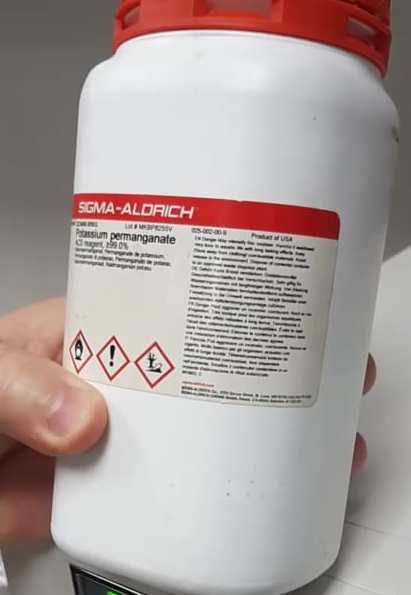
\includegraphics[width=0.3\textwidth]{Tarea1/muestras.png}
    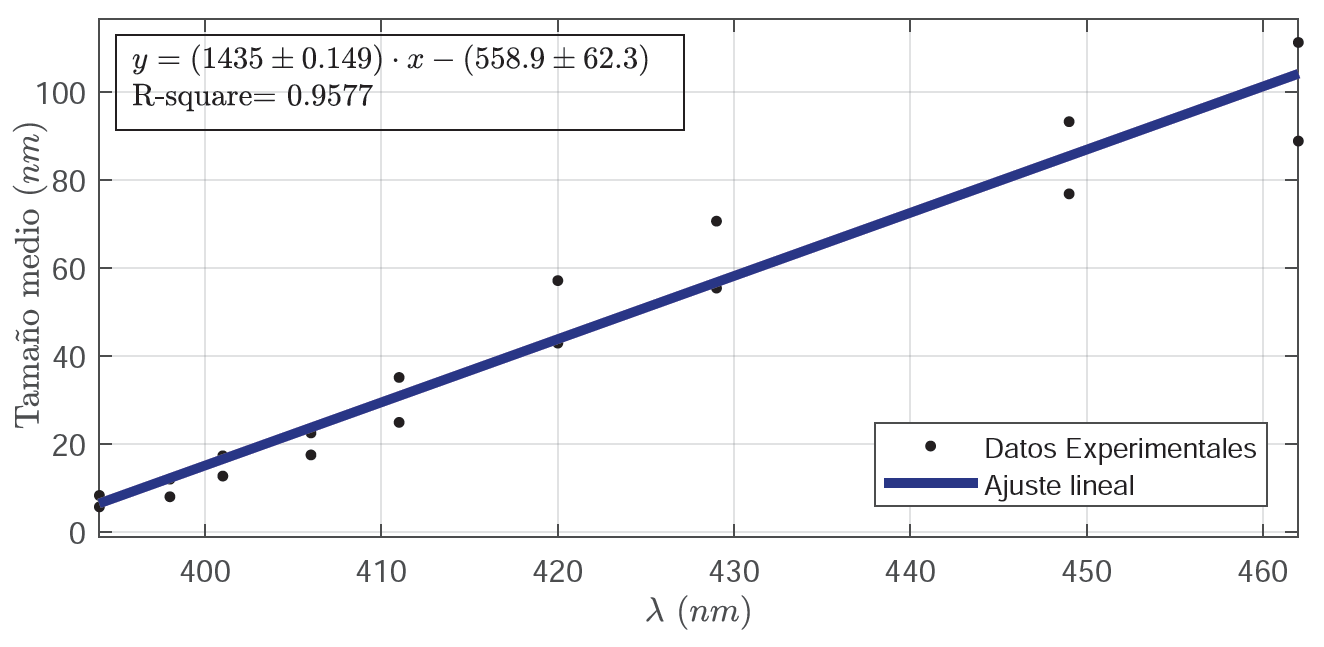
\includegraphics[width=0.49\textwidth]{Tarea3/tamano_experimental.png}
    \caption{\textbf{Ajuste lineal a valores experimentales a $pH=10$.}}
    \label{tamano}
\end{figure}


Ahora, el agente reductor citrato trisódico ($TSC$) contribuye a la formación de nano partículas con una distribución de tamaños mas grandes. También puede dar variación a la variación en la forma de las nanopartículas. Entonces, utilizando cualquiera de los agentes reductores, puede ser difícil sintetizar las nanopartículas de plata, por encima de $50~ nm$ y por debajo de $10~nm$ que tiene una forma bien definida con la monodispersidad deseada. El método de reducción conjunta que emplea dos reductores diferentes (es decir, $NaBH4$ y $TSC$) puede ofrecer un mejor control sobre la nucleación y el crecimiento de las nanopartículas $7,26$. Esto puede ayudar en la síntesis de diferentes tamaños de $AgNPs$ utilizando ligeras variaciones en el mismo protocolo.

\textbf{\textcolor{azul50}{Procedimiento Experimental}}

Aca se presentarán los procedimientos para la obtencion de los compuestos a caracterizar en el laboratorio:

\textbf{Síntesis de nanopartículas de plata.}

Primeramente se realizó la obtención de las nanopartículas de plata, para esto vertemos en un matraz, $250~ml$ de agua que que se agitará continuamente a una temperatura de $\approx 60^o$, agregamos $5~ml$ de trisodio citrato ($Na_3C_6H_5O_7$) con concentración de $0.5~mM$, despues de una espera de $1~min$, agregamos $2~ml$ de nitrato de plata ($AgNO_3$) con concentración de $0.2~mM$, despues de una espera de $5~min$, agregamos $0.5~ml$ de borihidruro de sodio ($NaBH_4$) con concentración de $2~mM$.

\textbf{Estudio de $AgNPs$ para diferentes $pH$.}

Se caracterizarán las nanopartículas de plata $AgNPs$ a diferentes valores de pH, los cambios se realizarán con los compuestos  $NaOH$ y $HCl$, para aumentar y bajar respectivamente el pH de nuestra muestra de nanopartículas, las mediciones de pH se realizarán con el "HI 2210 pH Meter Hanna" (medidor de pH mostrado en la Fig. \ref{ph}). Nuestro objetivo es medir nuestro valor inicial de pH (localizado en la Tabla 4 por una $*$) y obtener 3 muestras para pH mayores y 4 muestras para pH menores, los valores de pH resultantes serán mostrados en la Tabla 4, además, muestras de $200~\mu l$ serán recogidas con las micropipetas correspondiente a cada uno de ellos y puesta en la microplaca para su estudio con un espectrofotómetro como el mostrado en la Fig. \ref{espectro} para un barrido desde $350~nm-650~nm$.

\textbf{Estudio de $AgNPs$ mezcladas en diferentes proporciones con sales de $NaCl$ y $H_2O$.}

Con el objetivo de caracterizar muestra mezcla $AgNPs$ con diferentes concentraciones de sales ($NaCl$) y agua ($H_2O$) se realizarán preparados con porcentajes que varían desde $0\%-100\%$ con un paso de $10\%$, de estos $200~\mu l$ serán recogidas con las micropipetas correspondiente a cada uno de ellos y puesta en la microplaca para su estudio con un espectrofotómetro con barridos desde $350~nm-650~nm$ para la onda monocromática.

\textbf{\textcolor{azul50}{Obtención y análisis de Resultados}}

Se procederá a analizar los datos obtenidos por el espectrofotómetro de los compuestos anteriormente obtenidos.

\textbf{Estudio de $AgNPs$ para diferentes $pH$.}

Se prepararon 8 muestras con diferentes pH, estas obtenidos realizando cambios en la introducción de los compuestos de $NaOH$ y $HCl$, los valores de pH reportados por el "HI 2210 pH Meter Hanna" se muestran en la Tabla 4, estos fueron procesados por el programa matlab2017b y graficados como se muestra en la Fig. \ref{diff_pH}.

\textbf{Tabla 4: Valores de los picos máximo de los gráficos de $Absorbancia~vs~\lambda~(nm)$ en muestras de $AgNPs$ con diferentes $pH$.}

\begin{tabular}{|c|c|c|c|c|}
    \hline
    pH &  2.46 & 6 & 7 & 8 \\
    \hline
    $\lambda(A_{\max})$ & 391 & 397 & 396.6 & 395.8\\
    \hline\hline
    pH & 9.88 $^*$& 11.35 & 11.96 & 12.29\\
    \hline
    $\lambda(A_{\max})$ & 396.5 & 397 & 391 & 390\\
    \hline
\end{tabular}

Al procesar los datos se pudo notar que para los valores extremos $pH~=~2.46$ y $pH~=~12.29$ los gráficos de $A~vs~\lambda ~(nm)$ ya no muestran comportamientos esperados para mezclas con nanopartículas, se podría suponer la destrucción de estás para estos valores extremales. Para los valores intermedios de $pH$ se pudo notar el comportamiento esperado, solo con ligeras variaciones del pico máximo (Ver Figs. \ref{diff_pH})a y \ref{diff_pH})b.

Con la intención de localizar los valores extremos en los gráficos de $A~vs~\lambda ~(nm)~vs~pH$ se presenta la necesidad de encontrar los gráficos de $\partial A/\partial \lambda~vs~\lambda$ para los compuestos con diferentes $pH$ (Ver Fig. \ref{diff_pH}c). La localización se realizó interceptando el gráfico $\partial A/\partial \lambda~vs~\lambda$ con el plano $\partial A/\partial \lambda = 0$ (Ver Fig. \ref{diff_pH}), de está manera se obtuvieron los $\lambda$ para los máximos de absorbancia haciendo uso del matlab2017b, estos fueron introducidos en la Tabla 4 haciéndolos corresponder con sus respectivos $pH$. 

Al analizar estos valores, tenemos que las variaciones de estos valores cumplen con la condición $ \|\overline{ \lambda (A_{\max}) }  - \lambda ( A_{\max})\|~ < ~\Delta\lambda=3 ~nm$  (Error instrumental + Error de simulación = 1 $nm$ + 2 $nm$) los gráficos de $A~vs~\lambda (nm)$ por lo que no es posible diferenciar cambios de los $\lambda$ correspondiente a los picos para los gráficos con diferentes $pH$, de aqui que $\overline{ \lambda ( A_{\max} )} \approx (395.5\pm 3.0)~nm$, según la literatura, los picos correspondientes a este valor se relacionan con el tamaño medio de las nanopartículas (Ver Fig. \ref{tamano}) el cual está dado por 
$\overline{d} \approx  (1.43\pm 0.15)\cdot  \overline{ \lambda ( A_{\max} )} -(559\pm 62)\approx (7.48\pm 0.86)~n m$.

\begin{figure}
    %\centering
    %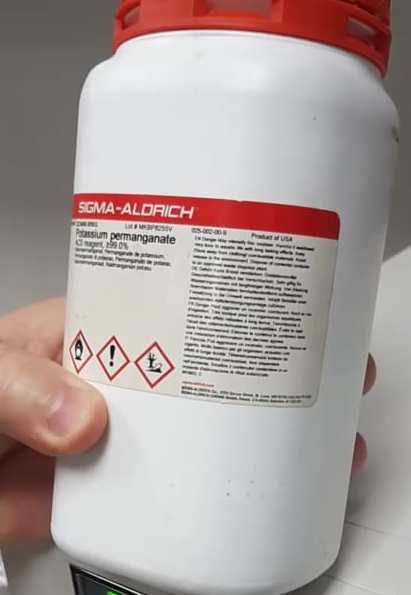
\includegraphics[width=0.3\textwidth]{Tarea1/muestras.png}
    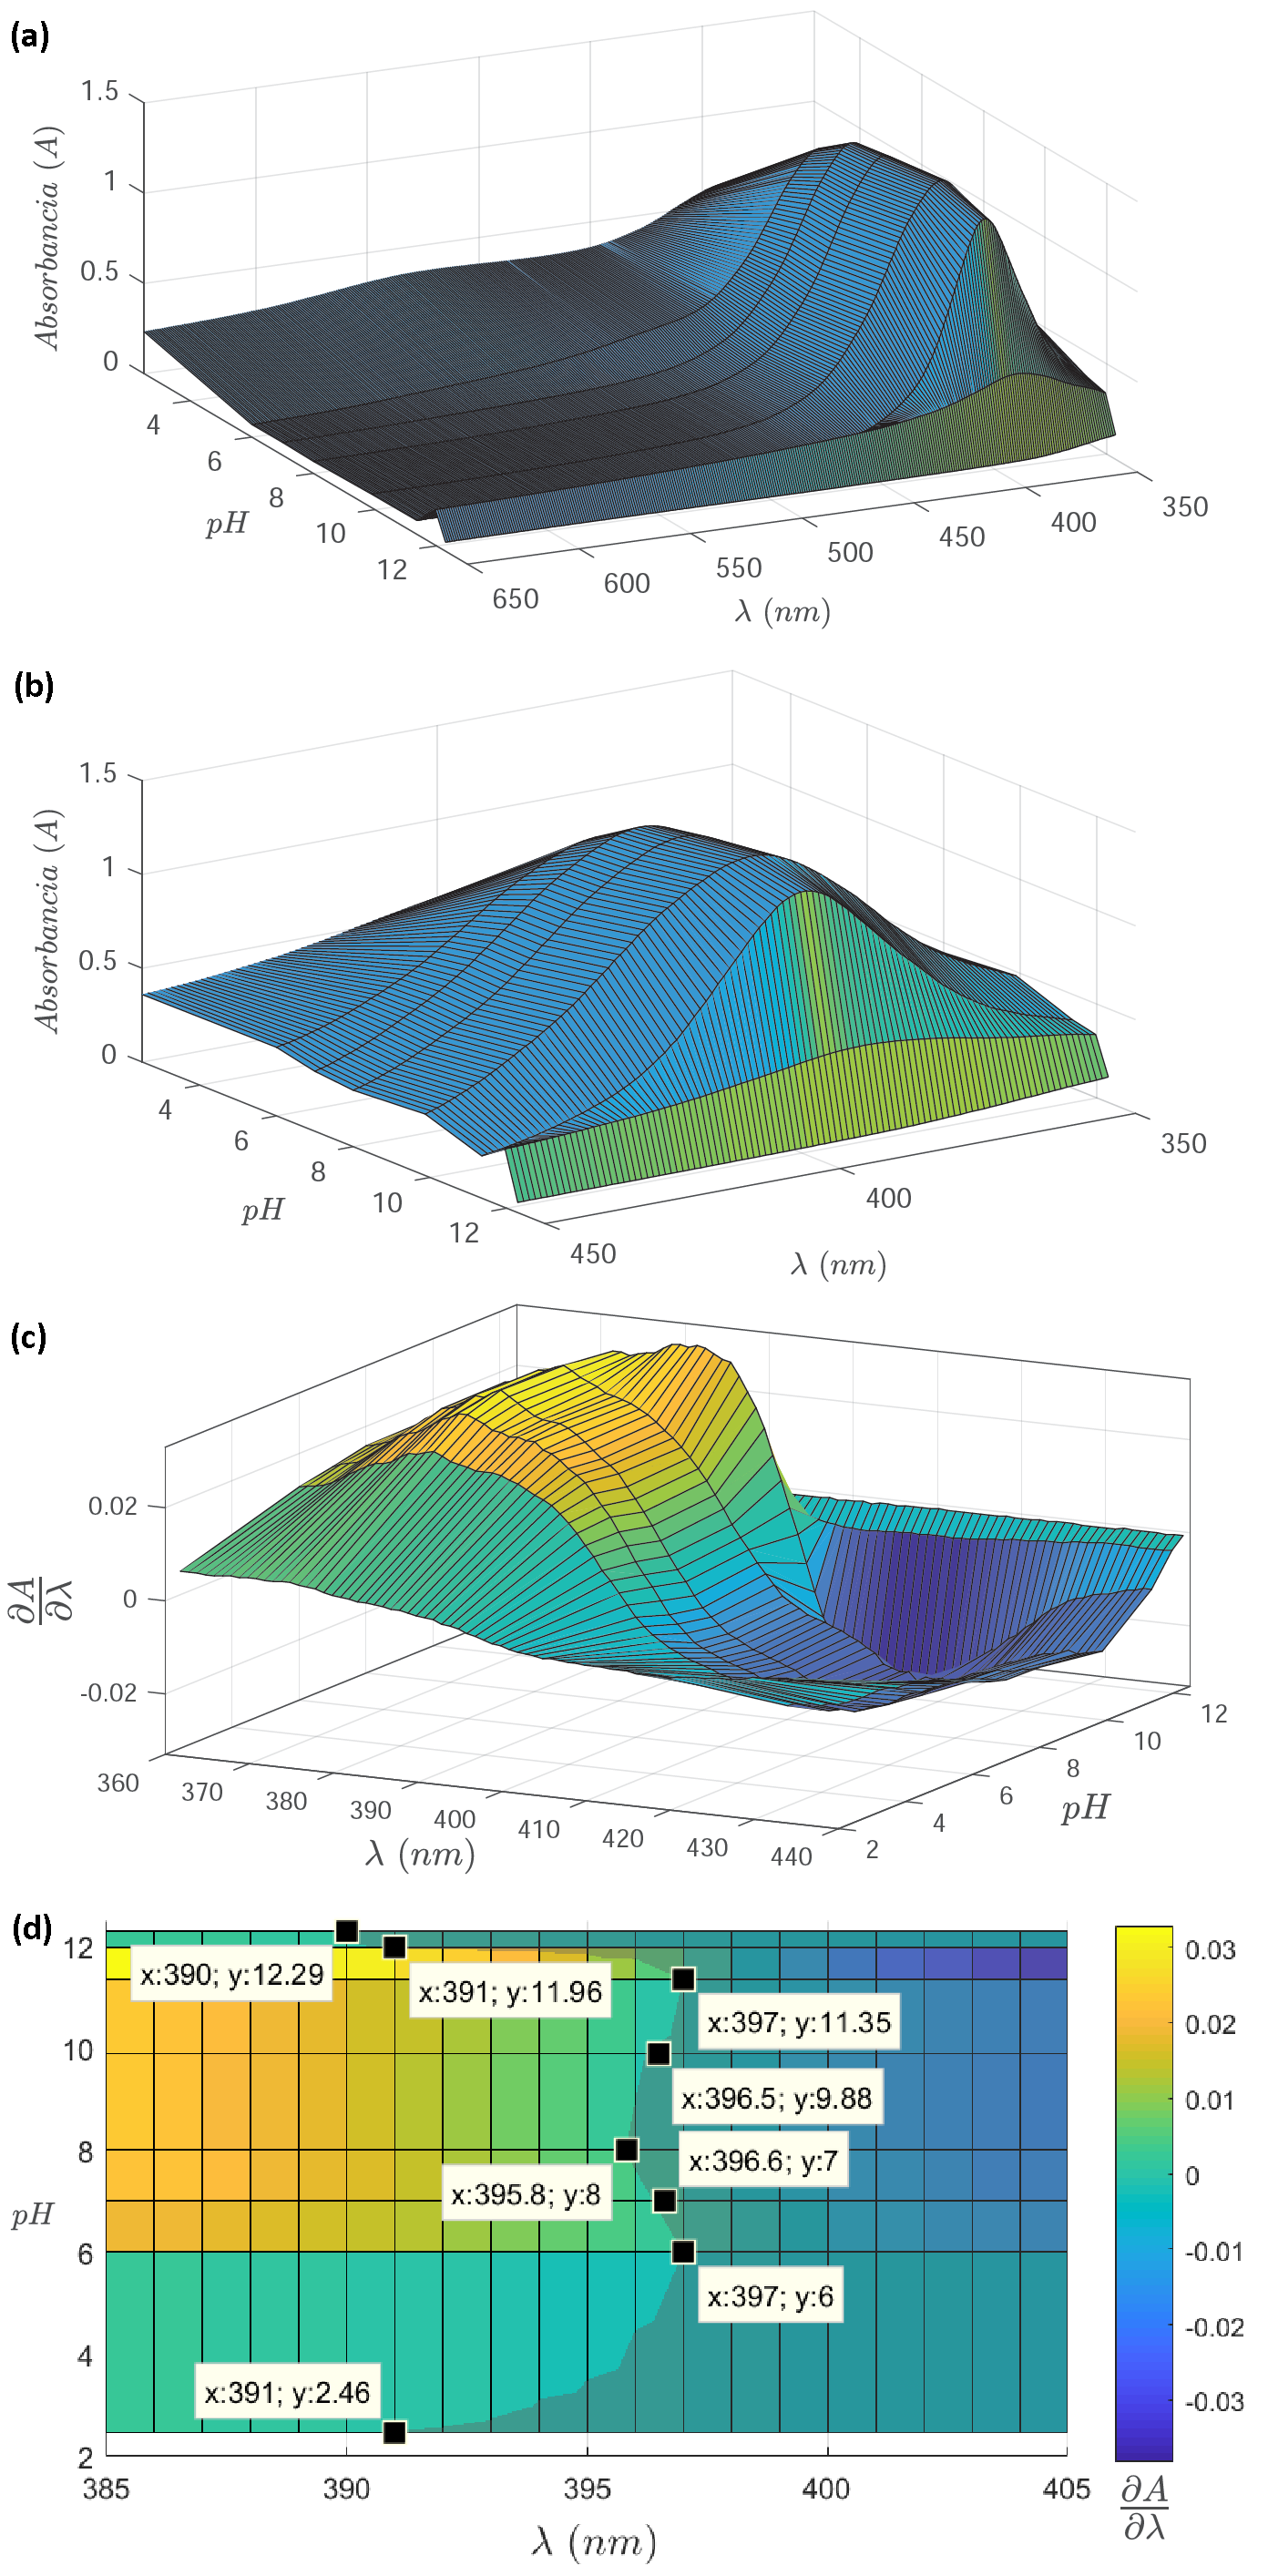
\includegraphics[width=0.49\textwidth]{Tarea3/AgNPs_pH.png}
    \caption{\textbf{Procesamiento de los datos de $AgNPs$ con diferentes $pH$.}}
    \label{diff_pH}
\end{figure}
También en las Figs. \ref{diff_pH}a y \ref{diff_pH}b se puedo apreciar cambios en la altura de esos picos, pero estos cambios no fueron procesados ni serán analizados.

\textbf{Estudio de $AgNPs$ mezcladas en diferentes proporciones con sales de $NaCl$.}

Siguiendo la línea de caracterización en la sección de procedimiento experimental se procesaron los gráficos obtenidos con el espectrofotómetro pero para muestras con diferentes proporciones entre las nanopartículas de plata $AgNPs$ y las sales $NaCl$, las mismas se muestran en las Figs. \ref{nacl}a y \ref{nacl}b. En estas se evidencia la presencia de dos comportamientos superpuestos, típico de la presencia  predominante de dos tamaños medios en nuestra muestra y los mismos se corresponden para todo el barrido caracterizado.

Semejante a los analisis anteriores caracterizaremos los gráficos de $A(\lambda)$ pero a diferentes concentración de $NaCl$, específicamente se procedió a caracterizar los máximos locales de nuestro conjuntos de muestras, para esto se implementó el gráfico relativo a $\partial A/\partial \lambda(\lambda,NaCl)$ (Ver Fig. \ref{nacl}c). El primer grupo de máximos (valores de $\lambda(A_{\max})$) se localizó interceptando el gráfico $\partial A/\partial \lambda(\lambda,NaCl)$ con el plano $\partial A/\partial \lambda =0$, los resultados se muestran en la Tabla 5.

En condiciones normales si tuvieramos la forma matemática específica de los gráficos de $A(\lambda)$ para diferentes muestras de nanopartículas de conocido tamaño podriamos realizar una superposición de los gráficos y encontrar mediante simulación el pico del segundo grupo de nanoparticulas de menos porcentaje de aparición, por cuestiones técnicas y operativas se consideró suficiente solo tener un valor cercano al real de este maximo $\lambda(A_{\max}^2)$, el mismo fue obtenido tratando el gráfico de $\partial^2 A/\partial \lambda^2 (\lambda,NaCl)$ al interceptalo con el plano $\partial^2 A/\partial \lambda^2=0$ en la zona esperada de esta irregularidad (Ver Fig. \ref{nacl}d), los resultados se tabularon en la Tabla 5 haciendolos corresponder son la respectiva proporción del valor de $NaCl$ en muestro compuesto.

\textbf{Tabla 5: Valores de los picos máximo de los gráficos de $Absorbancia~vs~\lambda~(nm)$ en muestras de $AgNPs$ mezcladas con $NaCl$ en diferentes proporciones.}

\begin{tabular}{|c|c|c|c|c|c|}
    \hline
    $NaCl$ &  $0\%$ & $10\%$ & $20\%$ & $30\%$ & $40\%$ \\
    \hline
    $\lambda(A_{\max})$ & $391.5$ & $392$ & $392.2$ & $396.8$ & $392.4$\\
    \hline
    $\lambda(A_{\max}^2)$ & $414.6$ & $414.7$ & $414.6$ & $420.7$ & $414.6$\\
    \hline\hline
    $NaCl$  & $50\%$ & $60\%$ & $70\%$ & $80\%$ & $90\%$ \\
    \hline
    $\lambda(A_{\max})$ & $391.9$ & $391.8$ & $392.9$ & $392.6$ & $393$\\
    \hline
    $\lambda(A_{\max}^2)$ & $414.6$ & $414$ & $416.9$ & $417.5$ & $421$\\
    \hline
\end{tabular}

Al analizar los datos de la Tabla 5, tenemos un caso atípico para una proporción del $30\%$ para el $NaCl$, tanto para los resultados de $\lambda (A_{\max})$ y $\lambda (A_{\max}^2)$, dado la poca cantidad de casos presentados y la no correspondencia con el resto de los valores solo podemos asumir que sea un error humano en algún momento de implementado el procedimiento de caracterización, y que como resultado se haya contaminado el compuesto, por lo cual desechamos este gráfico para los análisis siguientes.

\begin{figure}
    %\centering
    %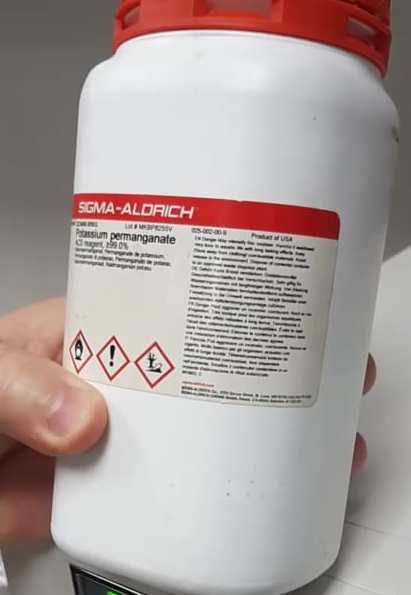
\includegraphics[width=0.3\textwidth]{Tarea1/muestras.png}
    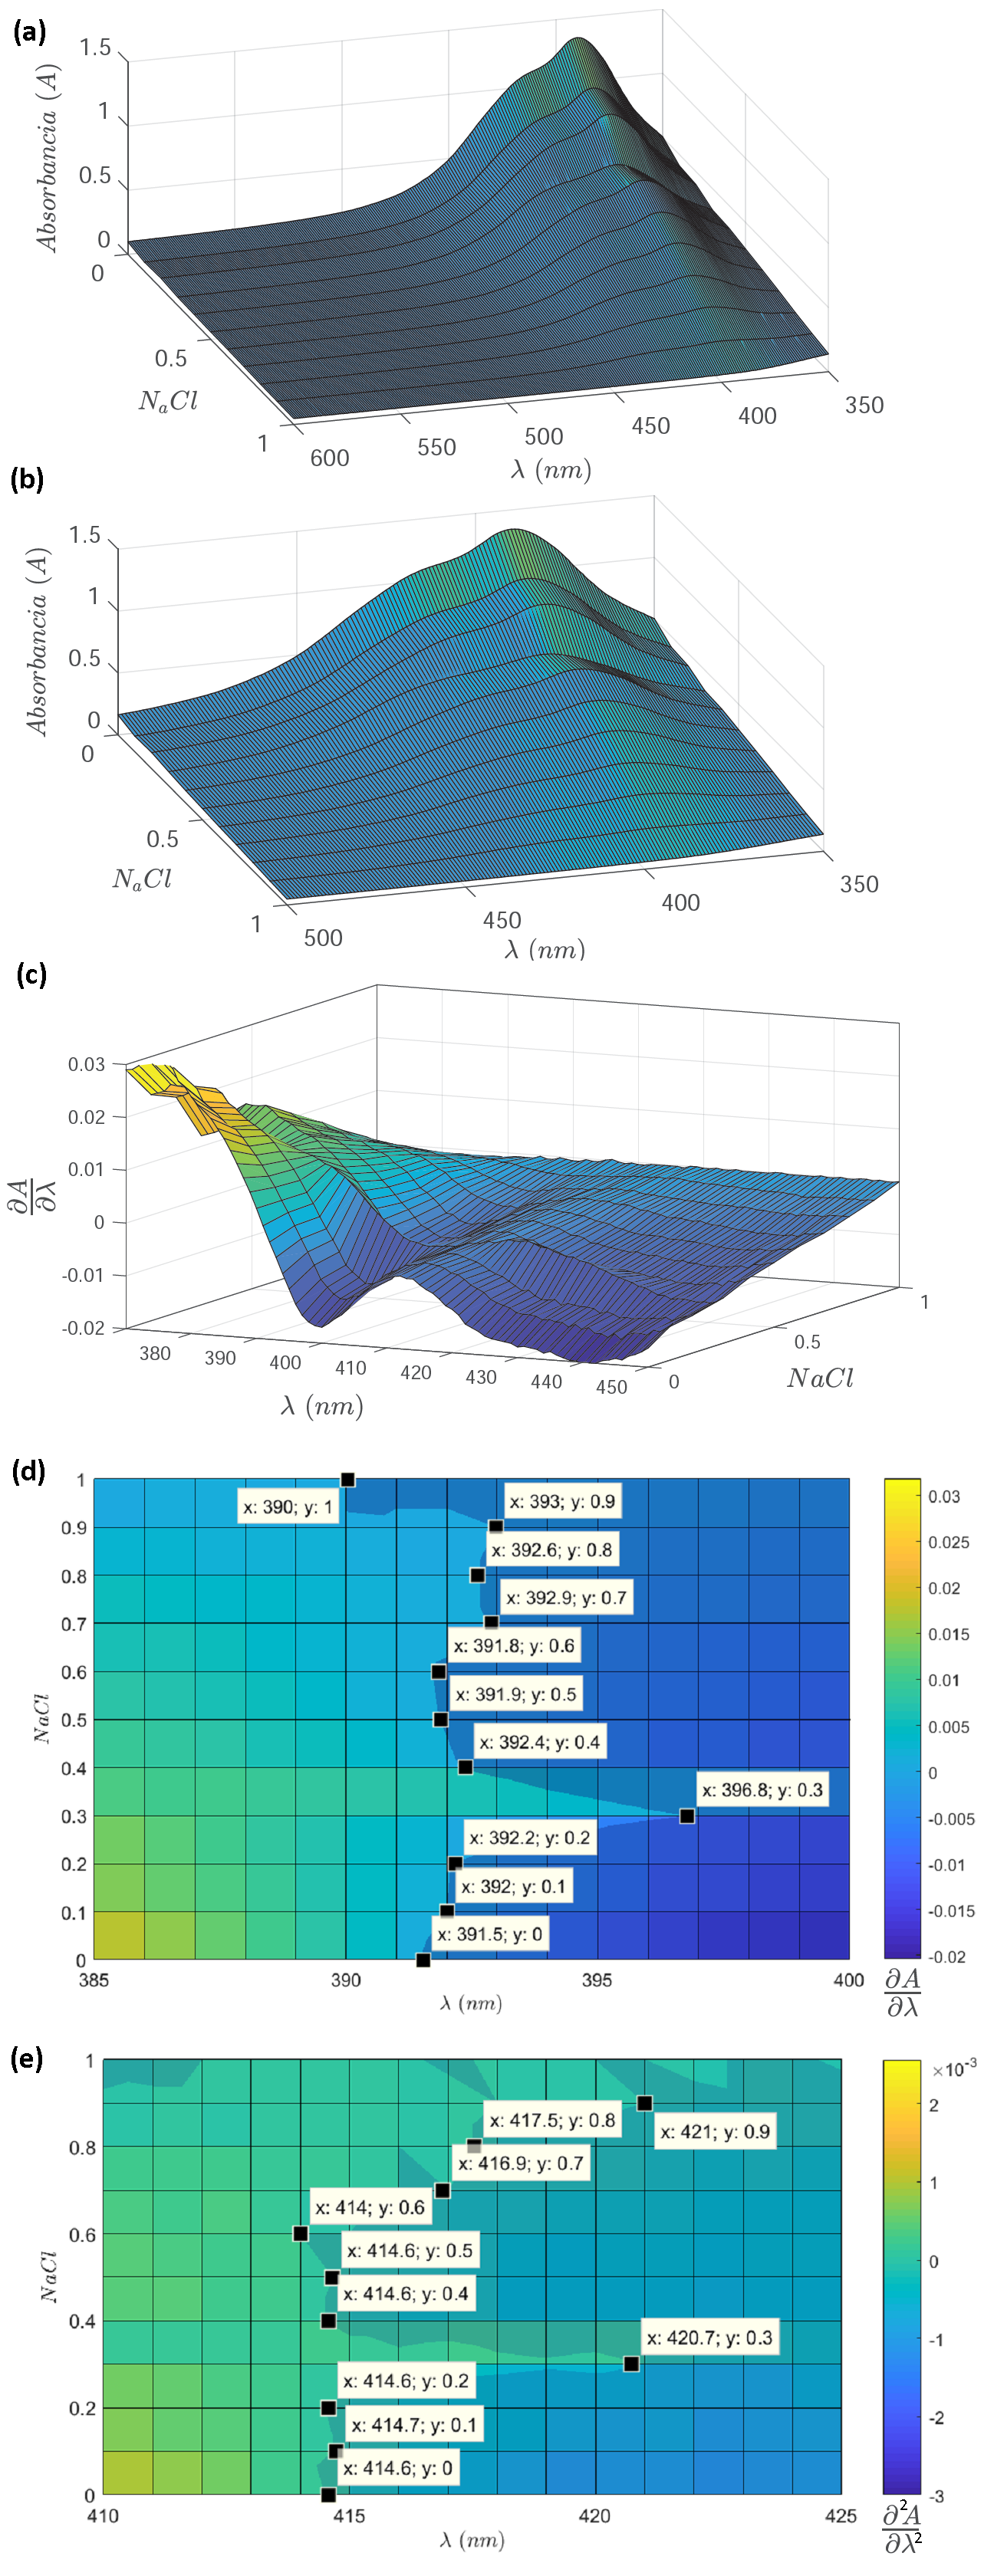
\includegraphics[width=0.47\textwidth]{Tarea3/AgNPs_NaCl.png}
    \caption{\textbf{Procesamiento de los datos de $AgNPs$ con diferentes concentración de $NaCl$.}}
    \label{nacl}
\end{figure}

Exceptuando al correspondiente caso atípico, tenemos que las variaciones de estos valores cumplen con la condición $ \|\overline{ \lambda (A_{\max}) }  - \lambda ( A_{\max})\|~ < ~\Delta\lambda=3 ~nm$  (Error instrumental + Error de simulación = 1 $nm$ + 2 $nm$) y que $ \|\overline{ \lambda (A_{\max}^2) }  - \lambda ( A_{\max}^2)\|~ < ~\Delta\lambda=4 ~nm$  (Error instrumental + Error de simulación = 1 $nm$ + 3 $nm$), el aumento del error de simulación está relacionado con los filtros que se aplicaron para procesar los datos en el programa matlab2017b, estos aumentan la incertidumbre de los resultados a obtener.

Al visualizar los resultados de $\lambda (A_{\max})$ y $\lambda (A_{\max}^2)$ obtenidos de los gráficos de $A~vs~\lambda (nm)$ se visualizaron cambios menores a los errores de nuestros datos por lo que no es posible diferenciar cambios de los $\lambda$ correspondiente a los picos principales buscados, de aqui que $\overline{ \lambda ( A_{\max} )} \approx (392.3\pm 3.0)~nm$, $\overline{ \lambda ( A_{\max}^2 )} \approx (415.8\pm 4.0)~nm$.

Haciendo uso de los resultados mostrados en la literatura, los picos correspondientes a los valores $\overline{ \lambda ( A_{\max} )}$ y $\overline{ \lambda ( A_{\max}^2)}$ se relacionan con el tamaño medio de las nanopartículas (Ver Fig. \ref{tamano}), los cuales están dados por:

$\overline{d} \approx  (1.43\pm 0.15)\cdot  \overline{ \lambda ( A_{\max} )} -(559\pm 62)\approx (3.6\pm 0.46)~n m$ 

$\overline{d_2} \approx  (1.43\pm 0.15)\cdot  \overline{ \lambda ( A_{\max}^2)} -(559\pm 62)\approx (37.2\pm 5.4)~n m$.

\textbf{Estudio de $AgNPs$ mezcladas en diferentes proporciones con sales de $H_2O$.}

Realizando un análisis semejante a los compuestos con sales se procesarán los gráficos obtenidos con el espectrofotómetro pero para muestras con diferentes proporciones entre las nanopartículas de plata $AgNPs$ y agua $H_2O$, las mismas se muestran en las Figs. \ref{h2o}a y \ref{h2o}b. En estas se evidencia la presencia de comportamiento típico de nanopartículas para concentraciones de agua de $\leq 30\%$, en caso contrario en los gráficos no se identifica los mismos y se asume la destrución de las nanopartículas para esas concentraciones, estos gráficos no serán procesados en la caracterización siguiente.

Se caracterizarán los gráficos de $A~vs~\lambda ~(nm)$ pero a diferentes concentración de $H_2O$, específicamente se procedió a caracterizar los máximos locales de nuestro conjuntos de muestras, para esto se implementó el gráfico relativo a $\partial A/\partial \lambda~vs~\lambda~vs~H_2O$ (Ver Fig. \ref{h2o}c). Los máximos (valores de $\lambda(A_{\max})$) se localizarón con la intercepción del gráfico $\partial A/\partial \lambda~vs~\lambda~vs~H_2O$ con el plano $\partial A/\partial \lambda =0$ (Ver Fig. \ref{h2o}d), los resultados se muestran en la Tabla 6.

\textbf{Tabla 6: Valores de los picos máximo de los gráficos de $Absorbancia~vs~\lambda~(nm)$ en muestras de $AgNPs$ mezcladas con $H_2O$ en diferentes proporciones.}

\begin{tabular}{|c|c|c|c|c|c|}
    \hline
    $H_2O$ &  $0\%$ & $10\%$ & $20\%$ & $30\%$ \\
    \hline
    $\lambda(A_{\max})$ & $392.1$ & $395.3$ & $396$ & $395$\\
    \hline
\end{tabular}

Al comparar los resultados obtenidos se notan diferencias marcadas con las muestras mezcladas con sales $NaCl$, para las muestras con agua no se mostraron evidencia de un segundo grupo de partículas, pero si de la traslación del pico principal de absorción a valores de $\lambda$ mayores cuando se comparan los resultados de $\lambda(A_{\max})$ para $H_2O$ a $0\%$ y los compuestos con agua ($H_2O$ a $>0\%$).

Al analizar los datos de la Tabla 5, se muestran que los resultados para $\lambda (A_{\max})$ son pocos, por lo que no es posible hacer una correspondencia entre ellos. Además, no se evidencia cambio en la posición de los picos, para los compuestos con agua $H_2O>0\%$ ya que tenemos que las variaciones de estos valores cumplen con la condición $ \|\overline{ \lambda (A_{\max}) }  - \lambda ( A_{\max})\|~ < ~\Delta\lambda=3 ~nm$  (Error instrumental + Error de simulación = 1 $nm$ + 2 $nm$), de aqui que se tratará con los valores medios $\overline{ \lambda ( A_{\max} )} \approx (395.4\pm 3.0)~nm$. 

\begin{figure}
    %\centering
    %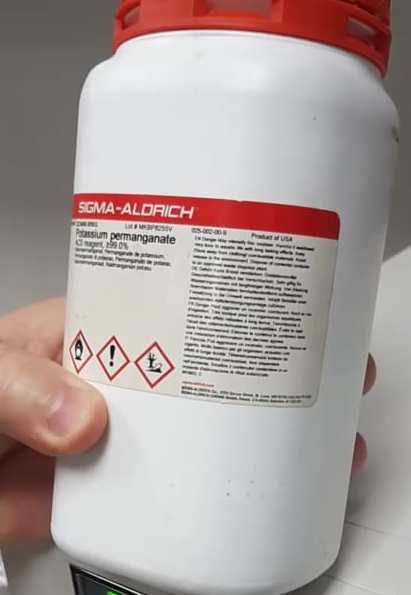
\includegraphics[width=0.3\textwidth]{Tarea1/muestras.png}
    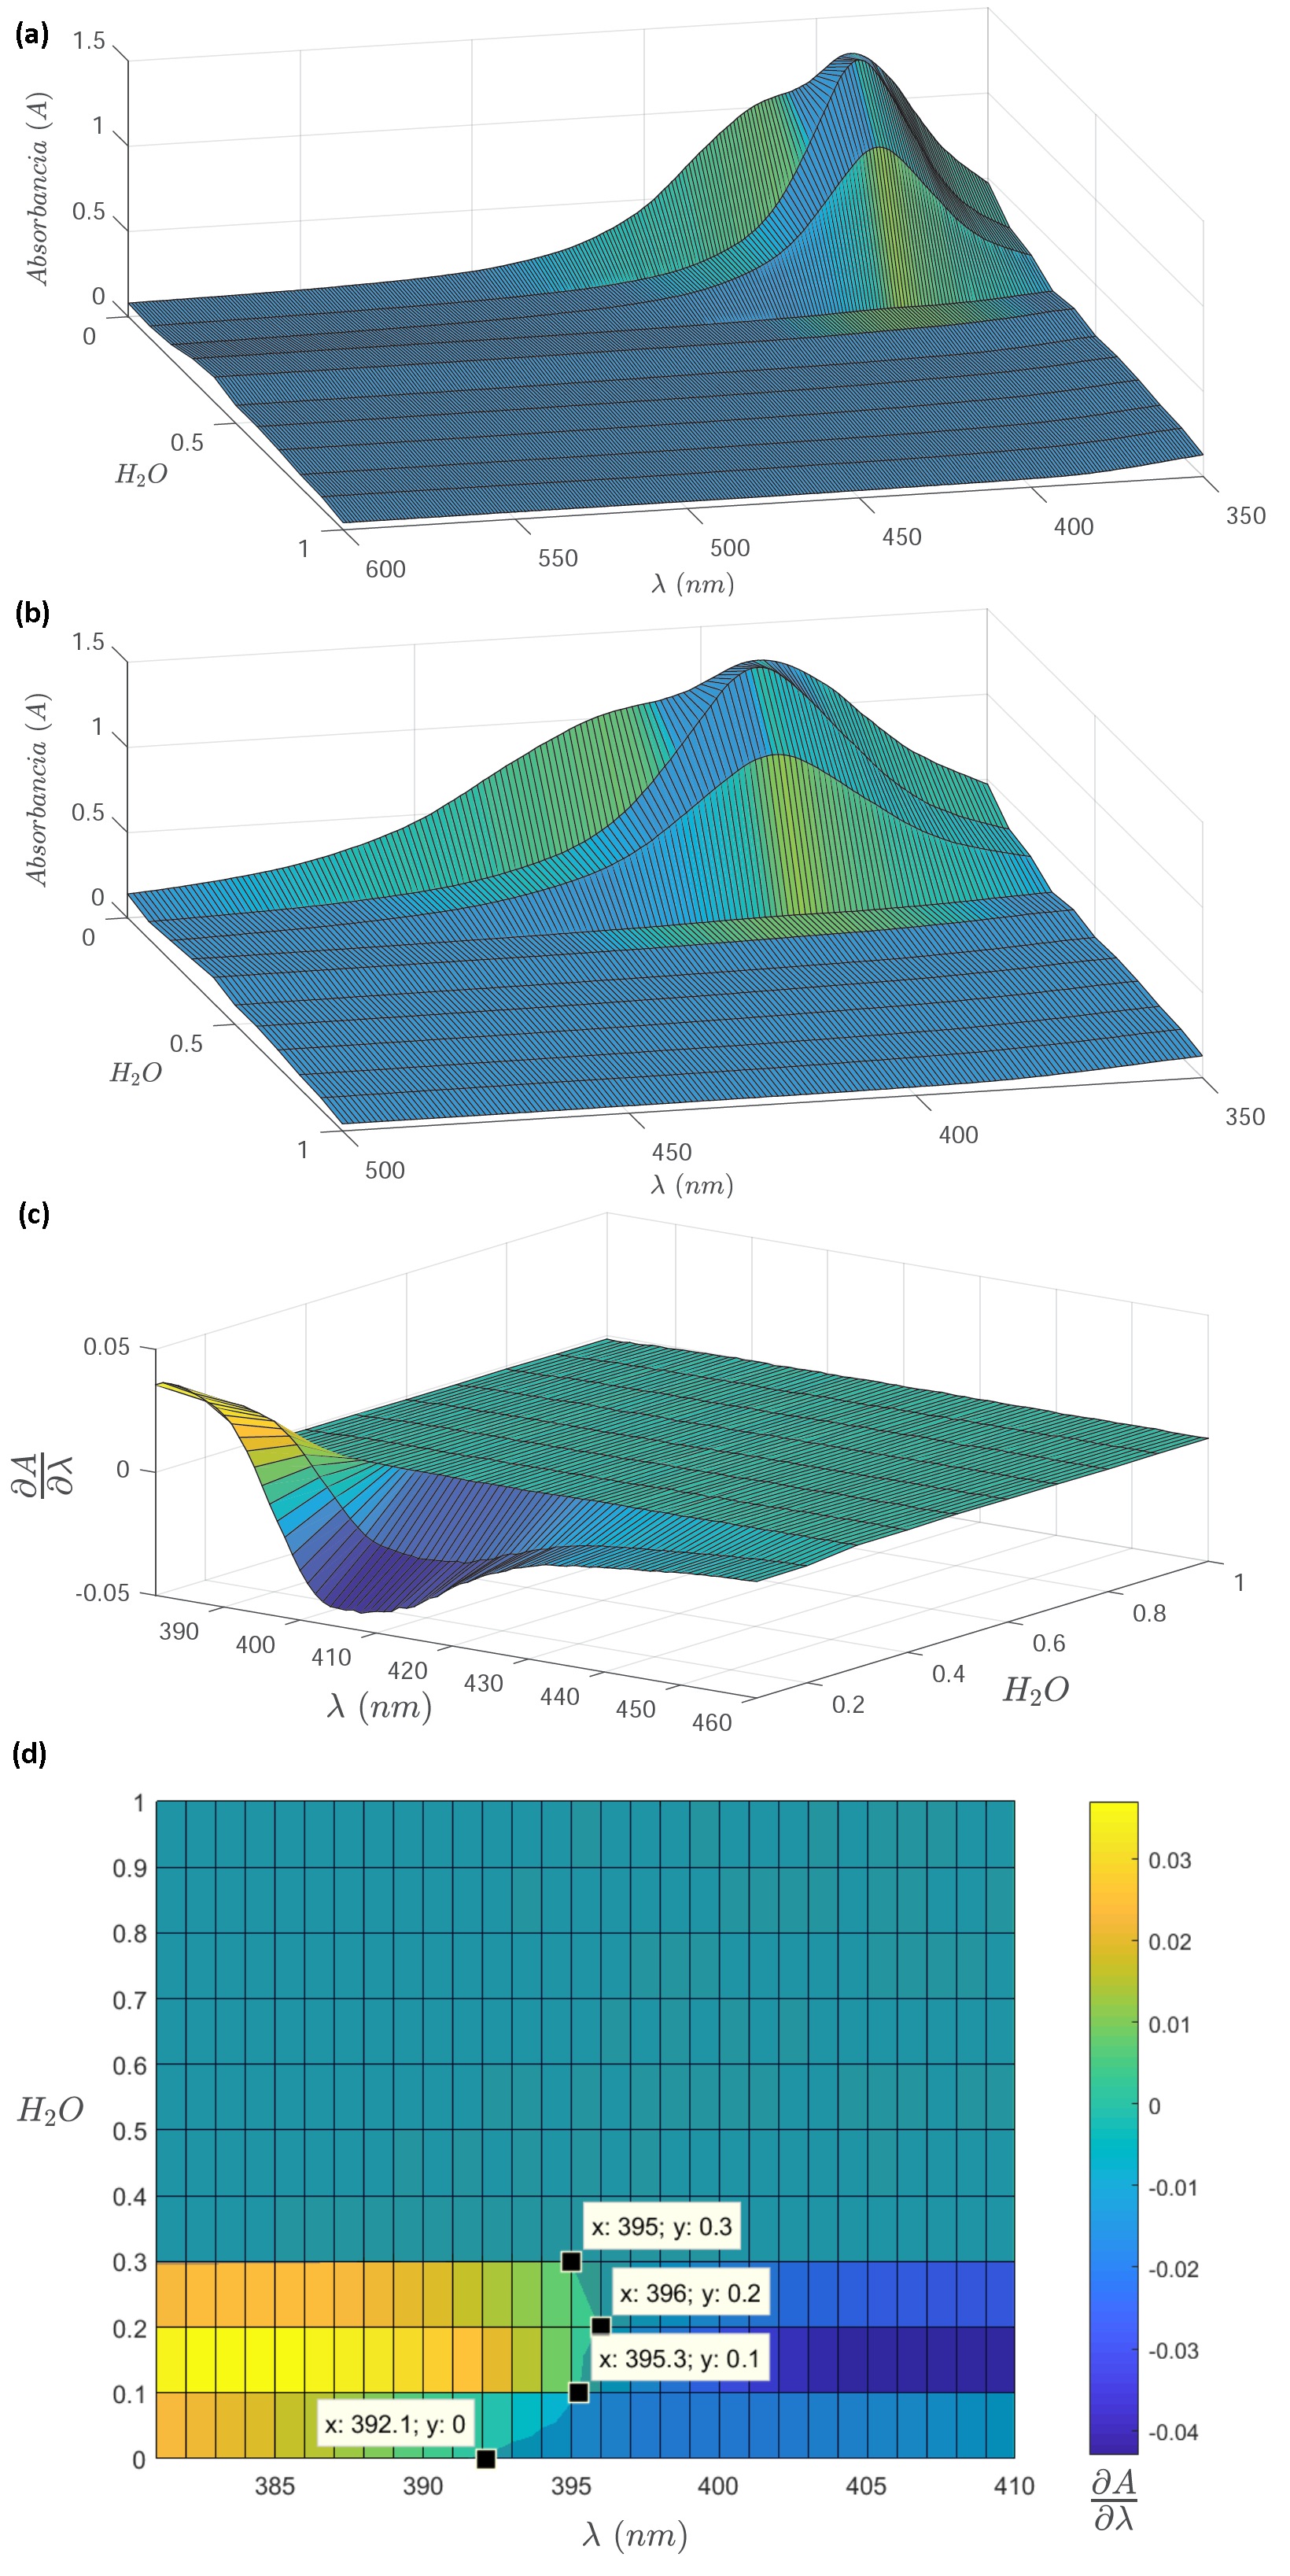
\includegraphics[width=0.49\textwidth]{Tarea3/AgNPs_H2O.png}
    \caption{\textbf{Procesamiento de los datos de $AgNPs$ con diferentes concentración de $H_2O$.}}
    \label{h2o}
\end{figure}

Haciendo uso de los resultados mostrados en la literatura, los picos correspondientes a los valores $\overline{ \lambda ( A_{\max} )}$ se relacionan con el tamaño medio de las nanopartículas (Ver Fig. \ref{tamano}), por lo cual podemos suponer que poseemos nanopartículas con tamaño medio de:

$\overline{d} \approx  (1.43\pm 0.15)\cdot  \overline{ \lambda ( A_{\max} )} -(559\pm 62)\approx (8.05\pm 0.91)~n m$

\textbf{\textcolor{azul50}{Conclusiones}}

En este laboratorio se trabajaron compuestos de nanopartículas de plata $AgNPs$, en los mismos se logró evaluar la estabilidad de nuestro compuesto ante diferentes condiciones de $pH$, o al ser mezclado con $NaCl$ y $H_2O$, se logró encontrar un valor aproximado de los valores de tamaño de grano para cada uno de nuestros compuestos y pudimos comprobar la diferencia en estos valores. Con el análisis de nuestros datos se da por cumplido la pláctica.





